% New Commands ------------------------------------------
\newcommand{\graficarDatosMio}[6]{
  \begin{tikzpicture}
  \begin{axis}[
      title={#1},
      xlabel={#2},
      ylabel={#3},
      scaled x ticks=false,
      scaled y ticks=false,
      width=0.6\textwidth
  ]
  \addplot[only marks, color=black] table[x=#4,y=#5]{#6};
  \end{axis}
\end{tikzpicture}
}

\newcommand{\graficarDatosSinOutliers}[8]{
  \begin{tikzpicture}
  \begin{axis}[
      title={#1},
      xlabel={#2},
      ylabel={#3},
      scaled x ticks=false,
      scaled y ticks=false,
      width=0.6\textwidth,
      ymin=#7,
      ymax=#8,
      restrict y to domain=#7:#8
  ]
  \addplot[only marks, color=black] table[x=#4,y=#5]{#6};
  \end{axis}
\end{tikzpicture}
}

% End New Commands ------------------------------------------

\begin{figure}[h]
\begin{center}
\includegraphics[scale=0.2]{imagenes/dakar.jpg}
\end{center}
\end{figure}

\subsection{Problema a resolver}

El problema a resolver consiste en elegir que vehículo usar para cada etapa de un Rally Dakar ($n$ etapas), teniendo en cuenta que las posibilidades son: una BMX, una motocross o un buggy arenero, y la cantidad de veces que podemos utilizar los últimos dos es limitada ($K_m$ y $K_b$ respectivamente.).

Para cada etapa, el tiempo que nos toma realizarla varía dependiendo de que vehículo elijamos. La elección de los vehículos para las diferentes etapas debe ser tal que minimice el tiempo total.

\begin{itemize}
\item Ejemplo 1:

\begin{codesnippet}
2 etapas, 0 etapas máximo con la motocross, 1 etapa máximo con el buggy
etapa 1:
    - BMX: 6 minutos
    - motocross: 2 minutos
    - buggy: 3 minutos
etapa 2:
    - BMX: 2 minutos
    - motocross: 3 minutos
    - buggy: 8 minutos
\end{codesnippet}
\item Solución del ejemplo 1:

\begin{codesnippet}
Tiempo total: 5 minutos
etapa 1: buggy - 3 minutos
etapa 2: BMX - 2 minutos
\end{codesnippet}
\item Ejemplo 2:

\begin{codesnippet}
5 etapas, 2 etapas máximo con la motocross, 1 etapa máximo con el buggy
etapa 1:
    - BMX: 10 minutos
    - motocross: 4 minutos
    - buggy: 3 minutos
etapa 2:
    - BMX: 15 minutos
    - motocross: 3 minutos
    - buggy: 6 minutos
etapa 3:
    - BMX: 6 minutos
    - motocross: 5 minutos
    - buggy: 5 minutos
etapa 4:
    - BMX: 7 minutos
    - motocross: 6 minutos
    - buggy: 2 minutos
etapa 5:
    - BMX: 12 minutos
    - motocross: 2 minutos
    - buggy: 6 minutos
\end{codesnippet}
\item Solución del ejemplo 2:

\begin{codesnippet}
Tiempo total: 21 minutos
etapa 1: buggy - 3 minutos
etapa 2: motocross - 3 minutos
etapa 3: BMX - 6 minutos
etapa 4: BMX - 7 minutos
etapa 5: motocross - 2 minutos
\end{codesnippet}
\end{itemize}

\subsection{Resolución planteada}

Al ser un problema de optimización, vamos a resolverlo usando la técnica algorítmica de \texttt{Programación Dinámica}.

Pero antes de desarrollar el algoritmo, veamos que el problema cumpla con los requisitos necesarios para que se pueda aplicar la técnica mencionada\footnote{Los requisitos necesarios son extraidos del libro: Introduction to Algorithms. Thomas H. Cormen, Charles E. Leiserson, Ronald L. Rivest, and Clifford Stein.The MIT Press, 2005}:

    \subsubsection{Subestructura Óptima}
    Como mostramos brevemente antes, una solución para un problema de $n$ etapas usando a lo sumo $i$ motos y $j$ buggies consiste en:
    \begin{itemize}
        \item Un vector de vehículos $V_{n,i,j}$ de tamaño $n$, donde $V_{n,i,j}[h]$ indica el vehículo elegido para la etapa $h$ en la solución.
        \item El tiempo total obtenido con los vehículos elegidos: $T_{n,i,j} = \sum_{h=1}^{n}{costo(V_{n,i,j}[h], h)}$. Donde $costo(v, h)$ es el costo de usar el vehículo $v$ en la etapa $h$.
    \end{itemize}

    Y una solución $V_{n,i,j}$ es optima si:
    $$(\forall\ W_{n,i,j})\ \sum_{h=1}^{n}{costo(V_{n,i,j}[h], h)} \leq \sum_{h=1}^{n}{costo(W_{n,i,j}[h], h)}$$

    Sean $V_{n,i,j}$, $V_{n-1,i-1,j}$, $V_{n-1,i,j-1}$ y $V_{n-1,i,j}$ soluciones optimas. Entonces:
    \begin{itemize}
        \item $V_{n,i,j}$ es la solución óptima para $n$ etapas usando a lo sumo $i$ motos y $j$ buggies.
        \item $V_{n-1,i,j}$ es la solución óptima para $n-1$ etapas usando a lo sumo $i$ motos y $j$ buggies.
        \item $V_{n-1,i-1,j}$ es la solución óptima para $n-1$ etapas usando a lo sumo $i-1$ motos y $j$ buggies.
        \item $V_{n-1,i,j-1}$ es la solución óptima para $n-1$ etapas usando a lo sumo $i$ motos y $j-1$ buggies.
    \end{itemize}

    Ahora, vamos a mostrar que la solución óptima $V_{n,i,j}$ contiene alguna de las soluciones óptimas $V_{n-1,i,j}$, $V_{n-1,i-1,j}$ o $V_{n-1,i,j-1}$.

    \begin{lemma}
        Dada una solución óptima $V_{i,j}$ (cuyo tiempo es $T_{n,i,j}$), o bien:
        \begin{enumerate}
            \item $T_{n,i,j} = T_{n-1,i,j} + costo(BMX, n)$ $\implies$ $T_{n-1,i,j}$ es el tiempo de la solución óptima $V_{n-1,i,j}$ para $n-1$ etapas usando a lo sumo $i$ motos y $j$ buggies, o bien
            \item $T_{n,i,j} = T_{n-1,i-1,j} + costo(MOTO, n)$ $\implies$ $T_{n-1,i-1,j}$ es el tiempo de la solución óptima $V_{n-1,i-1,j}$ para $n-1$ etapas usando a lo sumo $i-1$ motos y $j$ buggies, o bien
            \item $T_{n,i,j} = T_{n-1,i,j-1} + costo(BUGGY, n)$ $\implies$ $T_{n-1,i,j-1}$es el tiempo de la solución óptima $V_{n-1,i,j-1}$ para $n-1$ etapas usando a lo sumo $i$ motos y $j-1$ buggies.
        \end{enumerate}
    \end{lemma}
    \begin{proof}[Demostración]
        Planteamos los 3 casos posibles:
        \begin{enumerate}
            \item Si $V_{n,i,j}[n] = BMX \rightarrow V_{n-1,i,j} = \{V_{n,i,j}[1],\ \dots,\ V_{n,i,j}[n-1]\}$ es óptima.
            \item Si $V_{n,i,j}[n] = MOTO \rightarrow V_{n-1,i-1,j} = \{V_{n,i,j}[1],\ \dots,\ V_{n,i,j}[n-1]\}$ es óptima.
            \item Si $V_{n,i,j}[n] = BUGGY \rightarrow V_{n-1,i,j-1} = \{V_{n,i,j}[1],\ \dots,\ V_{n,i,j}[n-1]\}$ es óptima.
        \end{enumerate}

        \begin{enumerate}
            \item Antes que nada, sabemos que $V_{n-1,i,j}$ es válida porque al haber una $BMX$ en la última etapa de $V_{n,i,j}$ sabemos que al considerar las $n-1$ etapas tenemos a lo sumo $i$ motos y a lo sumo $j$ buggies.

            Ahora, por absurdo, supongamos que $V_{n-1,i,j}$ no es óptima, o sea que $\exists\ W_{n-1,i,j} = \{w_1,\ \dots,\ w_{n-1}\}$ tal que $T_{W} < T_{n-1,i,j}$.
            Si consideramos ahora $Z_{n,i,j} = \{w_1,\ \dots,\ w_{n-1},\ BMX\}$, vemos que es una solución valida para $n$ etapas, ya que $W$ tenía a lo sumo $i$ motos y a lo sumo $j$ buggies en sus $n-1$ etapas, y $Z$ agrega una $BMX$ en la etapa $n$.
            Pero entonces,
            \begin{equation*}
                \begin{aligned}
                    T_{Z} &= \sum_{h=1}^{n-1}{costo(W_{n-1,i,j}[h], h)} + costo(BMX,n) = T_{W} + costo(BMX,n) \\
                          &< T_{n-1,i,j} + costo(BMX,n) = \sum_{h=1}^{n-1}{costo(V_{n,i,j}[h], h)} + costo(BMX,n) \\
                          &= \sum_{h=1}^{n}{costo(V_{n,i,j}[h], h)} = T_{n,i,j}
                \end{aligned}
            \end{equation*}
            Absurdo, $V_{n,i,j}$ era óptima y $Z$ es una solución para $n$ etapas con a lo sumo $i$ motos y a lo sumo $j$ buggies que tiene un tiempo menor estricto.

            Luego, el absurdo viene de suponer que $V_{n-1,i,j}$ no es óptima.
            \item Analogamente al caso anterior, sabemos que $V_{n-1,i-1,j}$ es válida porque al haber una $MOTO$ en la última etapa de $V_{n,i,j}$ sabemos que al considerar las $n-1$ etapas tenemos a lo sumo $i-1$ motos y a lo sumo $j$ buggies.

            Ahora, por absurdo, supongamos que $V_{n-1,i-1,j}$ no es óptima, o sea que $\exists\ W_{n-1,i-1,j} = \{w_1,\ \dots,\ w_{n-1}\}$ tal que $T_{W} < T_{n-1,i-1,j}$.
            Si consideramos ahora $Z_{n,i,j} = \{w_1,\ \dots,\ w_{n-1},\ MOTO\}$, vemos que es una solución valida para $n$ etapas, ya que $W$ tenía a lo sumo $i-1$ motos y a lo sumo $j$ buggies en sus $n-1$ etapas, y $Z$ agrega una $MOTO$ en la etapa $n$, por lo que ahora tenemos a lo sumo $i$ motos.
            Pero entonces,
            \begin{equation*}
                \begin{aligned}
                    T_{Z} &= \sum_{h=1}^{n-1}{costo(W_{n-1,i-1,j}[h], h)} + costo(MOTO,n) = T_{W} + costo(MOTO,n) \\
                          &< T_{n-1,i-1,j} + costo(MOTO,n) = \sum_{h=1}^{n-1}{costo(V_{n,i,j}[h], h)} + costo(MOTO,n) \\
                          &= \sum_{h=1}^{n}{costo(V_{n,i,j}[h], h)} = T_{n,i,j}
                \end{aligned}
            \end{equation*}
            Absurdo, $V_{n,i,j}$ era óptima y $Z$ es una solución para $n$ etapas con a lo sumo $i$ motos y a lo sumo $j$ buggies que tiene un tiempo menor estricto.

            Luego, el absurdo viene de suponer que $V_{n-1,i-1,j}$ no es óptima.
            \item Idem caso 2.
        \end{enumerate}
    \end{proof}

    \subsubsection{Subproblemas superpuestos}

    Queremos mostrar que la solución óptima $V_{n,i,j}$ se obtiene a partir de las soluciones óptimas $V_{n-1,i,j}$, $V_{n-1,i-1,j}$ o $V_{n-1,i,j-1}$.

    \begin{lemma}
        Dadas las soluciones óptimas $V_{n-1,i,j}$, $V_{n-1,i-1,j}$ y $V_{n-1,i,j-1}$ (cuyos tiempos son $T_{n-1,i,j}$, $T_{n-1,i-1,j}$, $T_{n-1,i,j-1}$ respectivamente):
            $$T_{n,i,j} = min(T_{n-1,i,j} + costo(BMX, n), T_{n-1,i-1,j} + costo(MOTO, n), T_{n-1,i,j-1} + costo(BUGGY, n))$$
         Donde $T_{n,i,j}$ es el tiempo de la solución óptima $V_{n,i,j}$.
    \end{lemma}

    \begin{proof}[Demostración]
        Supongamos, por absurdo, que $V_{n,i,j}$ no es óptima. O sea que $\exists\ W_{n,i,j} = \{w_1,\ \dots,\ w_{n}\}$ tal que $T_{W} < T_{n,i,j}$.

        Ahora, hay solo 3 posibilidades para el vehículo en $W_{n,i,j}[n]$ (la $n$-esima etapa de $W_{n,i,j}$):
        \begin{enumerate}
            \item $W_{n,i,j}[n] = BMX$
            \item $W_{n,i,j}[n] = MOTO$
            \item $W_{n,i,j}[n] = BUGGY$
        \end{enumerate}

        Veamos que pasa en cada uno de ellos:
        \begin{enumerate}
             \item Sea $Z_{n-1,i,j} = \{w_1,\ \dots,\ w_{n-1}\}$ y sea $T_{Z}$ el tiempo de $Z_{n-1,i,j}$. Sabemos que $Z_{n-1,i,j}$ es una solución valida ya que como $W_{n,i,j}$ tiene a lo sumo $i$ motos y $j$ buggies en la $n$-esima etapa, y esa etapa tiene una $BMX$, entonces $W_{n,i,j}$ tiene a lo sumo $i$ motos y $j$ buggies en sus $n-1$ etapas restantes. Luego:
                 \begin{equation*}
                 \begin{aligned}
                     T_{W} &= \sum_{h=1}^{n}{costo(W_{n,i,j}[h], h)} = \sum_{h=1}^{n-1}{costo(W_{n,i,j}[h], h)} + costo(BMX, n) \\
                           &= T_{Z} + costo(BMX, n) < T_{n,i,j}
                 \end{aligned}
                 \end{equation*}
                 Pero como $T_{W}$ es menor que $T_{n,i,j}$, en particular es menor que $T_{n-1,i,j} + costo(BMX, n)$. Entonces:
                 \begin{equation*}
                 \begin{aligned}
                     T_{W} &= T_{Z} + costo(BMX, n) < T_{n-1,i,j} + costo(BMX, n) \\
                           &\iff T_{Z} < T_{n-1,i,j}
                 \end{aligned}
                 \end{equation*}
                 Absurdo, ya que partimos de que $T_{n-1,i,j}$ era el tiempo de la solución óptima $V_{n-1,i,j}$. Luego, el absurdo viene de suponer que $V_{n,i,j}$ no es óptima.
            \item Sea $Z_{n-1,i-1,j} = \{w_1,\ \dots,\ w_{n-1}\}$ y sea $T_{Z}$ el tiempo de $Z_{n-1,i-1,j}$. Sabemos que $Z_{n-1,i-1,j}$ es una solución valida ya que como $W_{n,i,j}$ tiene a lo sumo $i$ motos y $j$ buggies en la $n$-esima etapa, y esa etapa tiene una $MOTO$, entonces $W_{n,i,j}$ tiene a lo sumo $i-1$ motos y $j$ buggies en sus $n-1$ etapas restantes. Luego:
                \begin{equation*}
                \begin{aligned}
                    T_{W} &= \sum_{h=1}^{n}{costo(W_{n,i,j}[h], h)} = \sum_{h=1}^{n-1}{costo(W_{n,i,j}[h], h)} + costo(MOTO, n) \\
                          &= T_{Z} + costo(MOTO, n) < T_{n,i,j}
                \end{aligned}
                \end{equation*}
                Pero como $T_{W}$ es menor que $T_{n,i,j}$, en particular es menor que $T_{n-1,i-1,j} + costo(MOTO, n)$. Entonces:
                \begin{equation*}
                \begin{aligned}
                    T_{W} &= T_{Z} + costo(MOTO, n) < T_{n-1,i-1,j} + costo(MOTO, n) \\
                          &\iff T_{Z} < T_{n-1,i-1,j}
                \end{aligned}
                \end{equation*}
                Absurdo, ya que partimos de que $T_{n-1,i-1,j}$ era el tiempo de la solución óptima $V_{n-1,i-1,j}$. Luego, el absurdo viene de suponer que $V_{n,i,j}$ no es óptima.
            \item Analoga al caso 2.
   \end{enumerate}
\end{proof}

Como vimos en el \textbf{Lema 1.2}, para resolver un problema con $n$ etapas y con a lo sumo $i$ motos y $j$ buggies, necesitamos la solución óptima de los siguientes subproblemas:
\begin{enumerate}
	\item $n-1$ etapas, con a lo asumo $i$ motos y $j$ buggies.
    \item $n-1$ etapas, con a lo asumo $i-1$ motos y $j$ buggies.
    \item $n-1$ etapas, con a lo asumo $i$ motos y $j-1$ buggies.
\end{enumerate}

De la misma manera para resolver los subproblemas enumerados previamente, necesitamos la solución óptima de otros subproblemas. A continuación se detalla la dependencia de cada subproblema: \\

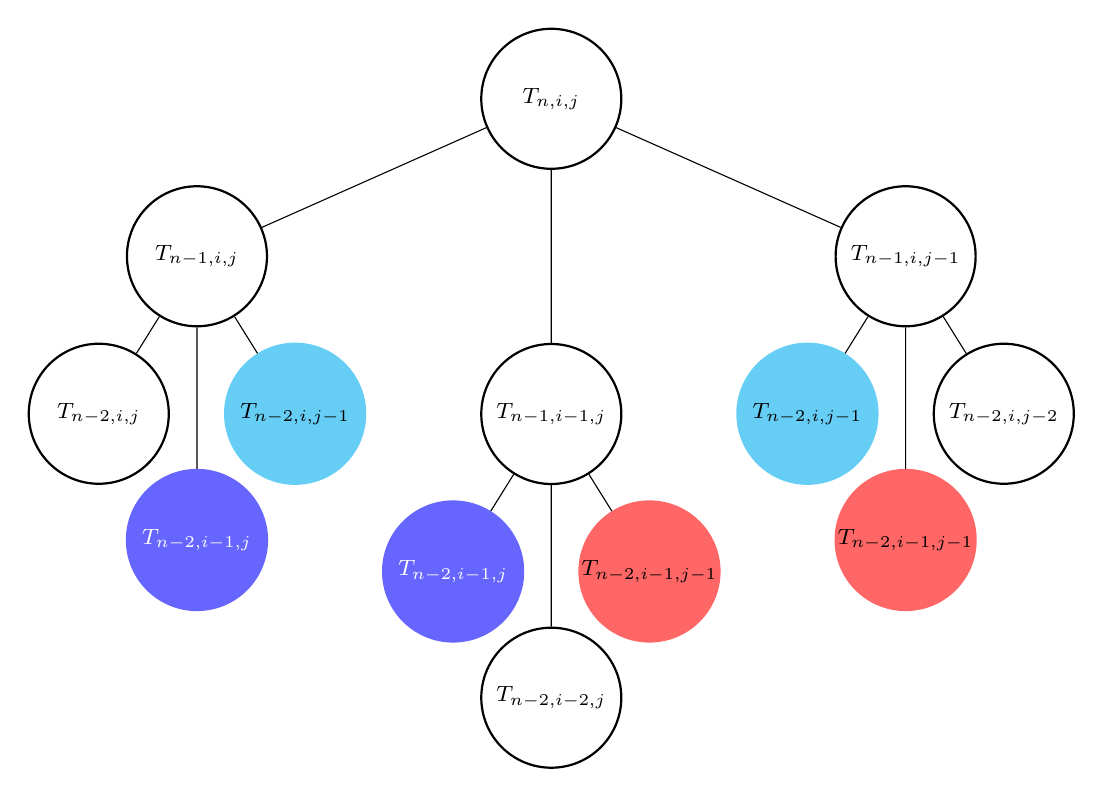
\begin{tikzpicture}[
   treenode/.style={align=center,fill=white,circle,draw=black,thick,inner sep=0, text width=5em, text centered, font=\footnotesize},
   treenode1/.style={align=center,circle,white, draw=blue!60, fill=blue!60, thick, inner sep=0, text width=5em, text centered, font=\footnotesize},
   treenode2/.style={align=center,circle,black, draw=red!60,fill=red!60,thick,inner sep=0, text width=5em, text centered, font=\footnotesize},
   treenode3/.style={align=center,circle,black, draw=cyan!60,fill=cyan!60,thick,inner sep=0, text width=5em, text centered, font=\footnotesize},
   level/.style={sibling distance = 4.5cm/#1,level distance = 2cm}
  ]
  \node[treenode] {$T_{n,i,j}$}
    child {node[treenode] {$T_{n-1,i,j}$}
      child {node[treenode, right=0.1cm] {$T_{n-2,i,j}$}}
      child {node[treenode1, below=0.7cm] {$T_{n-2,i-1,j}$}}
      child {node[treenode3, left=0.1cm] {$T_{n-2,i,j-1}$}}
    }
    child {node[treenode, below=1.1cm] {$T_{n-1,i-1,j}$}
      child {node[treenode1, right=0.1cm] {$T_{n-2,i-1,j}$}}
      child {node[treenode, below=0.7cm] {$T_{n-2,i-2,j}$}}
      child {node[treenode2, left=0.1cm] {$T_{n-2,i-1,j-1}$}}
    }
    child {node[treenode] {$T_{n-1,i,j-1}$}
      child {node[treenode3, right=0.1cm] {$T_{n-2,i,j-1}$}}
      child {node[treenode2, below=0.7cm] {$T_{n-2,i-1,j-1}$}}
      child {node[treenode, left=0.1cm] {$T_{n-2,i,j-2}$}}
    };
\end{tikzpicture}

Como surge de la imagen, hay subproblemas cuya solución es requerida por mas de un subproblema, generando una superposición de los mismos.
De esta manera, queda evidenciado la existencia de \textit{Subproblemas superpuestos} en este problema.

    \subsubsection{Formulación recursiva}

A continuación escribimos la solución del problema en términos de una función recursiva, donde $Km = i$ y $Kb = j$:

\begin{displaymath}
   T_{n,i,j} = \left\{
     \begin{array}{lr}
       costo(BMX,1) & : n = 1 \land i = 0 \land j = 0 \\
       min(costo(BMX,1), costo(MOTO,1))  & : n = 1 \land i > 0 \land j = 0  \\
       min(costo(BMX,1), costo(BUGGY,1))  & : n = 1 \land i = 0 \land j > 0  \\
       min(costo(BMX,1), costo(MOTO,1), costo(BUGGY,1) )  & : n = 1 \land i > 0 \land j > 0  \\
       T_{n-1,0,0} + costo(BMX,n) & : n > 1 \land i = 0 \land j = 0  \\
       min(T_{n-1,i,0} + costo(BMX,n), T_{n-1,i-1,0} + costo(MOTO,n)) & : n > 1 \land i > 0 \land j = 0  \\
       min(T_{n-1,0,j} + costo(BMX,n), T_{n-1,0,j-1} + costo(BUGGY,n)) & : n > 1 \land i = 0 \land j > 0  \\
       min(T_{n-1,i,j} + costo(BMX,n), T_{n-1,i-1,j} + costo(MOTO,n), & : n > 1 \land i > 0 \land j > 0 \\
                    \indent \indent T_{n-1,i,j-1} + costo(BUGGY,n))
     \end{array}
   \right.
\end{displaymath}

Habiendo justificado la utilización de la técnica algorítmica de \texttt{Programación Dinámica}, el algoritmo utilizado para resolver el problema, que sigue una estrategia bottom-up, se desarrolla de la siguiente forma:

\begin{itemize}
\item Creamos un vector \textit{costos} de tamaño igual a $n$, donde en el indice $i$ se almacenan los
      tiempos de la BMX, la moto y el buggy para la etapa $i$.

      \textit{Observación:} Los indices de las etapas a partir de ahora los vamos a representar de 0 a $n-1$, en vez de 1 a $n$ como veniamos haciendo. De esta forma esperamos que quede más claro la descripción del algoritmo, ya que coincide con la forma de acceder a las estructuras utilizadas.

\item Creamos un vector de matrices de tamaño $n*(Km+1)*(Kb+1)$ celdas, donde cada celda tiene atributos de \texttt{tiempo}, \texttt{vehículo} y \texttt{antecesor}, que nos permitiran más adelante reconstruir la solucion final.
\item Completamos la primera posición del vector de matrices (la primera etapa), de la siguiente manera:
  \begin{enumerate}
  	\item En la celda $(0,0,0)$ ponemos el costo del BMX para la etapa 0.
    \item Luego para el caso de la celda $(0,i,0)$ comparamos los costos para la etapa 0 de la BMX y de la MOTO, asignando al atributo \texttt{tiempo} el menor de ambos, y al atributo \texttt{vehículo} el vehículo correspondiente a ese costo, siendo el atributo \texttt{antecesor} un valor invalido debido a que estamos en la primera etapa. El caso $(0,0,j)$ es análogo.
    \item Para los casos donde $i,j > 0$, la comparación se debe hacer con los costos de todos los vehículos de la etapa 0, asignando a \texttt{tiempo} el tiempo menor de todos, y a \texttt{vehículo} el vehículo correspondiente a ese costo.
  \end{enumerate}
\item Luego, si tomamos una etapa $h$ cualquiera (con $0< h < n$) podemos completar de la siguiente forma:
  \begin{enumerate}
	\item En la celda $(h,0,0)$ ponemos el costo de la BMX para la etapa $h$ mas el tiempo en la celda $(h-1,0,0)$.
    \item Luego para el caso de la celda $(h,i,0)$ comparamos los costos para la etapa $h$ de la BMX mas el tiempo en la celda $(h-1,i,0)$ y de la MOTO en la etapa $h$ mas el tiempo en la celda $(h-1,i-1,0)$, asignando a \texttt{tiempo} el menor de ambos, y a \texttt{vehículo} el vehículo correspondiente a ese costo, siendo \texttt{antecesor} $(i,0)$ si el vehículo seleccionado es un BMX y $(i-1,0)$ si el vehículo seleccionado es una MOTO. El caso $(h,0,j)$ es análogo.
    \item Para los casos donde $i,j > 0$, comparamos los costos para la etapa $h$ de la BMX mas el tiempo en la celda $(h-1,i,j)$, de la MOTO en la etapa $h$ mas el tiempo en la celda $(h-1,i-1,j)$, y del BUGGY en la etapa $h$ mas el tiempo en la celda $(h-1,i,j-1)$  asignando a \texttt{tiempo} el costo menor de todos, y a \texttt{vehículo} el vehículo correspondiente a ese costo, y a \texttt{antecesor} $(i,j)$ si el vehículo seleccionado es un BMX, $(i-1,j)$ si el vehículo seleccionado es una MOTO, y $(i,j-1)$ si el vehículo seleccionado es un BUGGY.
  \end{enumerate}
  \item Al finalizar, el tiempo optimo lo obtenemos a partir de la posición $(n-1,i,j)$ y los vehículos correspondiente a cada etapa, los obtenemos a partir del antecesor de $(n-1,i,j)$, donde el $vehiculo[n-1]$ es igual al vehículo en $(n-1,i,j)$, $vehiculo[n-2]$ es igual al vehículo en el antecesor de $(n-1,i,j)$, y así sucesivamente hasta obtener los vehículos para cada etapa.
 \end{itemize}

 \subsubsection{Pseudocódigo}
En pseudocódigo nos queda:
\newline \newline
\begin{codesnippet}
Creamos una vector costos de tamaño igual a n, donde en el indice i se almacenan los
    tiempos de la bmx, la moto y el buggy para la etapa i-1.
Si Kb > n:
    Pongo Kb = n
Si Km > n:
    Pongo Km = n
Creamos un vector de matrices, infoEtapas, de n*(Km+1)*(Kb+1) celdas para almacenar
    las soluciones parciales.
Completamos la primera matriz del vector de la siguiente manera:
Para i = 0 hasta Km
    Para j = 0 hasta Kb
    	Si i = 0 y j = 0 entonces:
        	infoEtapas[0,0,0].tiempo = costo(BMX,0)
                infoEtapas[0,0,0].vehiculo = BMX
            Sino Si i = 0 entonces:
         	Si costo(BMX,0) < costo(BUGGY,0) entonces:
            	infoEtapas[0,0,j].tiempo = costo(BMX,0)
	            infoEtapas[0,0,j].vehiculo = BMX
		 Sino:
            	infoEtapas[0,0,j].tiempo = costo(BUGGY,0)
	            infoEtapas[0,0,j].vehiculo = BUGGY
             Sino Si j = 0 entonces:
         	Si costo(BMX,0) < costo(MOTO,0) entonces:
            	infoEtapas[0,i,0].tiempo = costo(BMX,0)
	            infoEtapas[0,i,0].vehiculo = BMX
	         Sino:
            	infoEtapas[0,i,0].tiempo = costo(MOTO,0)
		    infoEtapas[0,i,0].vehiculo = MOTO
             Sino:
                tBMX = costo(BMX,0)
                tMOTO = costo(MOTO,0)
                tBUGGY = costo(BUGGY,0)
        	Si tBMX < tMOTO y tBMX < tBUGGY  entonces:
            	infoEtapas[0,i,j].tiempo = tBMX
	            infoEtapas[0,i,j].vehiculo = BMX
	        Sino Si tMOTO < tBUGGY:
            	infoEtapas[0,i,j].tiempo = tMOTO
                    infoEtapas[0,i,j].vehiculo = MOTO
                Sino:
                   infoEtapas[0,i,j].tiempo = tBUGGY
	           infoEtapas[0,i,j].vehiculo = BUGGY
    Fin para todo
Fin para todo

  								(Continua)
\end{codesnippet}
\begin{codesnippet}
Completamos el resto de las matrices del vector:
Para h = 1 hasta n-1
	Para i = 0 hasta Km
    	Para j = 0 hasta Kb
        	Si i = 0 y j = 0 entonces:
            	infoEtapas[h,0,0].tiempo = infoEtapas[h-1,0,0].tiempo + costo(BMX,h)
                    infoEtapas[h,0,0].vehiculo = BMX
                    infoEtapas[h,0,0].antecesor = (0,0)
                Sino Si i = 0 entonces:
            	thBMX = infoEtapas[h-1,0,j].tiempo + costo(BMX,h)
                    thBUGGY = infoEtapas[h-1,0,j-1].tiempo + costo(BUGGY,h)
                    Si  thBMX < thBUGGY  entonces:
                	infoEtapas[h,0,j].tiempo = thBMX
    	            infoEtapas[h,0,j].vehiculo = BMX
                        infoEtapas[h,0,j].antecesor = (0,j)
                    Sino:
                	infoEtapas[h,0,j].tiempo = thBUGGY
    	            infoEtapas[h,0,j].vehiculo = BUGGY
                        infoEtapas[h,0,j].antecesor = (0,j-1)
                Sino Si j = 0 entonces:
                    thBMX = infoEtapas[h-1,i,0].tiempo + costo(BMX,h)
                    thMOTO = infoEtapas[h-1,i-1,0].tiempo + costo(MOTO,h)
             	Si costo(BMX,0) < costo(MOTO,0) entonces:
                	infoEtapas[h,i,0].tiempo = thBMX
    	            infoEtapas[h,i,0].vehiculo = BMX
                        infoEtapas[h,i,0].antecesor = (i,0)
    	        Sino:
                	infoEtapas[h,i,0].tiempo = thMOTO
    	            infoEtapas[h,i,0].vehiculo = MOTO
                        infoEtapas[h,i,0].antecesor = (i-1,0)
                Sino:
                    thBMX = infoEtapas[h-1,i,j].tiempo + costo(BMX,h)
                    thMOTO = infoEtapas[h-1,i-1,j].tiempo + costo(MOTO,h)
                    thBUGGY = infoEtapas[h-1,i,j-1].tiempo + costo(BUGGY,h)
            	Si thBMX < thMOTO y thBMX < thBUGGY  entonces:
                	infoEtapas[h,i,j].tiempo = thBMX
    	            infoEtapas[h,i,j].vehiculo = BMX
                        infoEtapas[h,i,j].antecesor = (i,j)
    	       Sino Si thMOTO < thBUGGY:
                	infoEtapas[h,i,j].tiempo = thMOTO
                        infoEtapas[h,i,j].vehiculo = MOTO
                        infoEtapas[h,i,j].antecesor = (i-1,j)
                  Sino:
                        infoEtapas[h,i,j].tiempo = thBUGGY
                        infoEtapas[h,i,j].vehiculo = BUGGY
                        infoEtapas[h,i,j].antecesor = (i,j-1)
           Fin para todo
      Fin para todo
 Fin para todo

Recontruimos la solución a partir de los antecesores
    de la posición infoEtapas[n-1,Km,Kb]

\end{codesnippet}

\subsection{Complejidad propuesta}

Como se desprende del pseudocódigo del punto anterior, el algoritmo que proponemos tiene 6 ciclos (uno simple, uno de 2 ciclos anidados y otro de 3 ciclos anidados). Vamos a verlos uno por uno:

\begin{enumerate}
	\item Completar el vector \textit{costos} con los costos de cada vehículo para cada etapa implica repetir la operación de almacenar datos $n$ veces, siendo la complejidad de la operación de almacenar constante por ser un vector para el cual reservamos $n$ posiciones. Por lo cual, la complejidad de este ciclo es de $\Theta(n)$.
    \item  Completar la primera matriz del vector \textit{infoEtapas} implica iterar $(Km+1)*(Kb+1)$ veces. Las operaciones dentro del ciclo son accesos, almacenamientos a un vector, y comparaciones, por lo cual todas las operaciones son constantes. Por lo tanto, la complejidad de este ciclo es de $\Theta((Km+1)*(Kb+1)) \in \Theta(Km*Kb)$.
     \item  Completamos el resto de las matrices del vector \textit{infoEtapas} lo cual implica iterar $(n-1)*(Km+1)*(Kb+1)$ veces. Las operaciones dentro del ciclo son accesos, almacenamientos a un vector, y comparaciones, por lo cual todas las operaciones son constantes. Por lo tanto, la complejidad de este ciclo es de $\Theta((n-1)*(Km+1)*(Kb+1)) \in \Theta(n*Km*Kb)$.
     \item El ultimo ciclo consiste en accesos a la infoEtapas para reconstruir el vector vehículos solución, desde la ultima posición. Para construir el vector vehículos solución iteramos $n$ veces, haciendo en cada iteración operaciones de costo constante. La complejidad de este ciclo es de $\Theta(n)$.

\end{enumerate}

Nos queda por ver las operaciones que están por fuera de los ciclos, las cuales son dos creaciones de vectores (uno para los \textit{costos} y otro para rearmar los \textit{vehiculos} de la solución final) y una creación de un vector de matrices. La creación de los vectores tiene una complejidad de $\Theta(n)$, mientras que la creación del vector de matrices tiene una complejidad de $\Theta((n-1)*(Km+1)*(Kb+1)) \in \Theta(n*Km*Kb)$.

A partir de lo que expusimos previamente, el calculo de complejidad es: $\Theta(n + Km*Kb + n*Km*Kb + n + n + n*Km*Kb + n)$, es decir $\Theta(n*Km*Kb) \in \mathcal{O}(n*Km*Kb)$ lo cual cumple con la complejidad temporal solicitada.

\newpage
\subsection{Implementación en C++}

\lstinputlisting[language=C++]{codigo/ej1.cpp}

\subsection{Experimentación computacional}
La función que utilizamos para llevar a cabo las mediciones fue \texttt{std::clock}\footnote{Referencia \url{http://en.cppreference.com/w/cpp/chrono/c/clock}}. La unidad temporal que utilizamos para este ejercicio fue nanosegundos.
La complejidad teórica calculada es de $\mathcal{O}(n*K_b*K_m)$

\subsubsection{Experimentación con instancias aleatorias}
Para generar las instancias aleatorias utilizamos la función \texttt{std::rand}\footnote{Referencia \url{http://en.cppreference.com/w/cpp/numeric/random/rand}} con determinados intervalos de valores para la variables, para obtener instancias coherentes. El detalle de intervalos es el siguiente:
\begin{itemize}
	\item Cantidad de etapas ($n$): 1 $\leq n \leq$ 100
    \item Costo maximo para bmx ($C_{bmx}$): 1 $\leq C_{bmx} \leq$ 1.000
    \item Cantidad de veces que se usa la Moto ($K_m$): 0 $\leq K_m \leq n$
    \item Cantidad de veces que se usa el Buggy ($K_b$): 0 $\leq K_b \leq n$
\end{itemize}

Generamos 100 instancias aleatorias para cada $n$, variando aleatoriamente el $K_m$ y el $K_b$ cada 10 muestras, luego promediadas. Su medición temporal, arroja el siguiente resultado:
\begin{center}
\graficarDatosMio
{Tiempos sin procesar, en nanosegundos}
{$n*K_m*K_b$}{Tiempo de ejecucion (nanosegundos)}
{n*km*kb}{nanosegundos}
{datos/ej1-datos1.dat}

\graficarDatosSinOutliers
{Dividiendo los tiempos por $n*K_m*K_b$}
{$n*K_m*K_b$}{Tiempo (nano sec.) / $n*K_m*K_b$}
{n*km*kb}{div-(n*km*kb)}
{datos/ej1-datos1.dat}
{0}{1000}
\end{center}

A continuación, adjuntamos una tabla con los últimos 20 valores obtenidos en las instancias aleatorias, teniendo en cuenta que los casos fueron previamente ordenados según el tamaño ($n$):

\begin{table}[H]
\parbox{0.3\textwidth}{
    \begin{tabular}{ | l | l | l | l | l |}
    \hline
	Etapas($n$)	&$K_m$	&$K_b$	&Tiempo(nanosegundos)	&Tiempo(nanosegundos) / ($n*K_m*K_b$)	\\ \hline
    99  &72  &37  &70072900.00  &265.69 \\ \hline
    99  &12  &73  &29759500.00  &343.15 \\ \hline
    99  &31  &7  &11082100.00  &515.85 \\ \hline
    99  &49  &81  &97282600.00  &247.58 \\ \hline
    99  &69  &45  &78407200.00  &255.06 \\ \hline
    99  &79  &87  &163650100.00  &240.51 \\ \hline
    99  &69  &21  &40036000.00  &279.09 \\ \hline
    99  &98  &59  &138501600.00  &241.95 \\ \hline
    99  &83  &17  &43269100.00  &309.75 \\ \hline
    99  &60  &89  &128942200.00  &243.90 \\ \hline
    100  &26  &40  &32398500.00  &311.52 \\ \hline
    100  &12  &17  &11816700.00  &579.25 \\ \hline
    100  &69  &37  &67029800.00  &262.55 \\ \hline
    100  &47  &19  &28339800.00  &317.35 \\ \hline
    100  &51  &19  &29314000.00  &302.51 \\ \hline
    100  &14  &49  &22309700.00  &325.21 \\ \hline
    100  &20  &78  &44039800.00  &282.30 \\ \hline
    100  &84  &49  &102553700.00  &249.15 \\ \hline
    100  &28  &99  &70483900.00  &254.27 \\ \hline
    100  &2  &66  &9976800.00  &755.81 \\ \hline
    \textbf{Promedio} &{} &{}  &6096330	&329.12 \\ \hline

    \end{tabular}
}
\end{table}

Como podemos ver de los gráficos y la tabla suministrada, al dividir los tiempos por $n*K_m*K_b$, tienden a un número constante mayor a cero. Entonces nuestro algoritmo tendría complejidad $\mathcal{O}(c*n*K_m*K_b)$, donde $c$ es la constante a la cual converge el gráfico. Por lo tanto concluimos que los gráficos se condicen con nuestra predicción de complejidad.

\subsubsection{Experimentación con instancias particulares}
Queda considerar la existencia o no de instancias particulares que afecten la ejecución del algoritmo, es decir si para una determinada combinación de valores de entrada cambia la complejidad del mismo.

A partir de un análisis del algoritmo, queda evidenciado que estas instancias no existen, ya que los ciclos que determinan la complejidad del mismo se ejecutan sin importar los valores particulares en los costos de cada vehículo por etapa. Por lo tanto, se concluye que no hay instancias particulares de mejor o peor caso para este algoritmo.